\section{Motor-Modell}

Das Motormodell besteht aus den drei Baugruppen Spannungs-Strom-Wandler, Gleichstrommotor und Getriebe. Die Modellierung der Baugruppen basiert auf den in Franke \cite{franke} erstmalig aufgestellten Gleichungen, die auch in den nachfolgenden Arbeiten zum Versuchsstand zur Anwendung kamen. Das Modell des Gleichstrommotors wird im Rahmen dieser Arbeit nun zusätzlich um die Berücksichtigung der Gegeninduktion des Motors erweitert.

\subsection{Spannungs-Strom-Wandler}

Bei dem am Versuchsstand eingesetzten Spannungs-Strom-Wandler handelt es sich um einen Servoverstärker, der ursprünglich zur Drehzahlregelung von Gleichstrommotoren vorgesehen war. Entsprechend folgt der Verstärker dem Prinzip einer übergeordneten Drehzahlregelung mit unterlagerter Stromregelung. Für die Anwendung am Versuchsstand ist der übergeordnete Drehzahlregelkreis jedoch aufgetrennt und in einen Spannungs-Strom-Wandler umfunktioniert worden. Dieser dient der Vorgabe eines konstanten Ankerstroms durch Pulsweitenmodulation (PWM) der Zwischenkreisspannung des Wandlers proportional zur eingehenden Steuerspannung. Das stationäre Verhalten kann aus diesem Grund durch einen Proportionalitätsfaktor $K_{UI}$ beschrieben werden
	\[
	I_a = K_{UI} \cdot U_{\mrm{Steuer}} \ .
\]

Gemäß Franke \cite{franke} lässt sich die Dynamik des Wandlers durch ein \mrm{PT_1}-Glied modellieren, sodass sich für den Wandler im Laplace-Bereich insgesamt die Gleichung
	\[
	I_a(s) = \frac{K_{UI}}{1+T_{UI} \cdot s} \cdot U_{\mrm{Steuer}}(s)
	\]
ergibt.


\subsection{Gleichstrommotor}

Bei dem verwendeten Motor handelt es sich um eine fremderregte Gleichstrommaschine, wobei die magnetische Erregung durch einen Permanentmagneten erzeugt wird \cite{franke}. Das elektromagnetische Drehmoment des Gleichstrommotors ist näherungsweise proportional zum Ankerstrom \cite{binder}. Hierbei wird vorausgesetzt, dass keine magnetische Sättigung vorliegt.
\[
	M_e = K_I \cdot I_a
\]

Neben dem elektromagnetischen Drehmoment sind außerdem parasitäre Reibmomente zu berücksichtigen. Die Modellierung der Reibung von Motor und Getriebe wird zusammen mit der Schlittenreibung in Kapitel \ref{sec:spdModell} behandelt. Ein rückwirkendes Moment durch die Federkraft des Riemens wird auf Grund der Annahme unendlicher Riemensteifigkeit vernachlässigt. 

Weiterhin wird das Drehmoment durch die Gegeninduktion geschwächt. Dieser Effekt ist in den Motormodellen von Franke \cite{franke} und den Nachfolgearbeiten bisher nicht berücksichtigt worden. Da die Erfahrung am realen Versuchsstand jedoch gezeigt hat, dass eine Modellierung der Gegeninduktion sinnvoll erscheint, wird diese im Rahmen dieser Arbeit in das Motormodell integriert.

Zum besseren Verständnis des Effekts wird zunächst das physikalische Prinzip der Gegeninduktion betrachtet. Fließt ein Strom durch den ruhenden Anker, der sich im Magnetfeld der Permanentmagneten befindet, so wirkt senkrecht zu den Richtungen des Stroms und des Magnetfelds die Lorenzkraft auf die in der Ankerwicklung befindlichen Ladungsträger (Drei-Finger-Regel bzw. Rechte-Hand-Regel in technischer Stromrichtung). Durch das entstehende Drehmoment beginnt der Anker zu rotieren. Durch die Drehung bewegen sich die Ladungsträger nun zusätzlich zur eigentlichen Stromrichtung auch in Rotationsrichtung des Ankers. Auf diese Bewegungskomponente kann nun erneut das Prinzip der Lorentzkraft angewendet werden. Die resultierende zusätzliche Kraftkomponente, die in Abhängigkeit der Rotationsgeschwindigkeit auf die Ladungsträger wirkt, zeigt nun gegen die Stromrichtung (Lenz'sche Regel). Der resultierenden Ladungsbeschleunigung kann ein Spannungsabfall über der Ankerwicklung zugeordnet werden, die sogenannte induzierte Gegenspannung oder Gegen-EMK (Gegen-Elektromagnetische-Kraft). Der in Folge sinkende Ankerstrom reduziert das Drehmoment des Motors. \cite{binder}

Am Versuchsstand wird dieser Effekt bei geringen Winkelgeschwindigkeiten durch den Stromregler des Spannungs-Strom-Wandlers kompensiert. Ab einer bestimmten Winkelgeschwindigkeit bei konstantem Sollstrom wird die induzierte Gegenspannung größer als die maximale Zwischenkreisspannung des Spannungs-Strom-Wandlers, sodass nicht mehr ausgeregelt werden kann. Nun nimmt der Ankerstrom und damit das Drehmoment mit steigender Winkelgeschwindigkeit ab bis die Leerlaufdrehzahl erreicht ist. 

\begin{figure}[htbp]
	\centering
		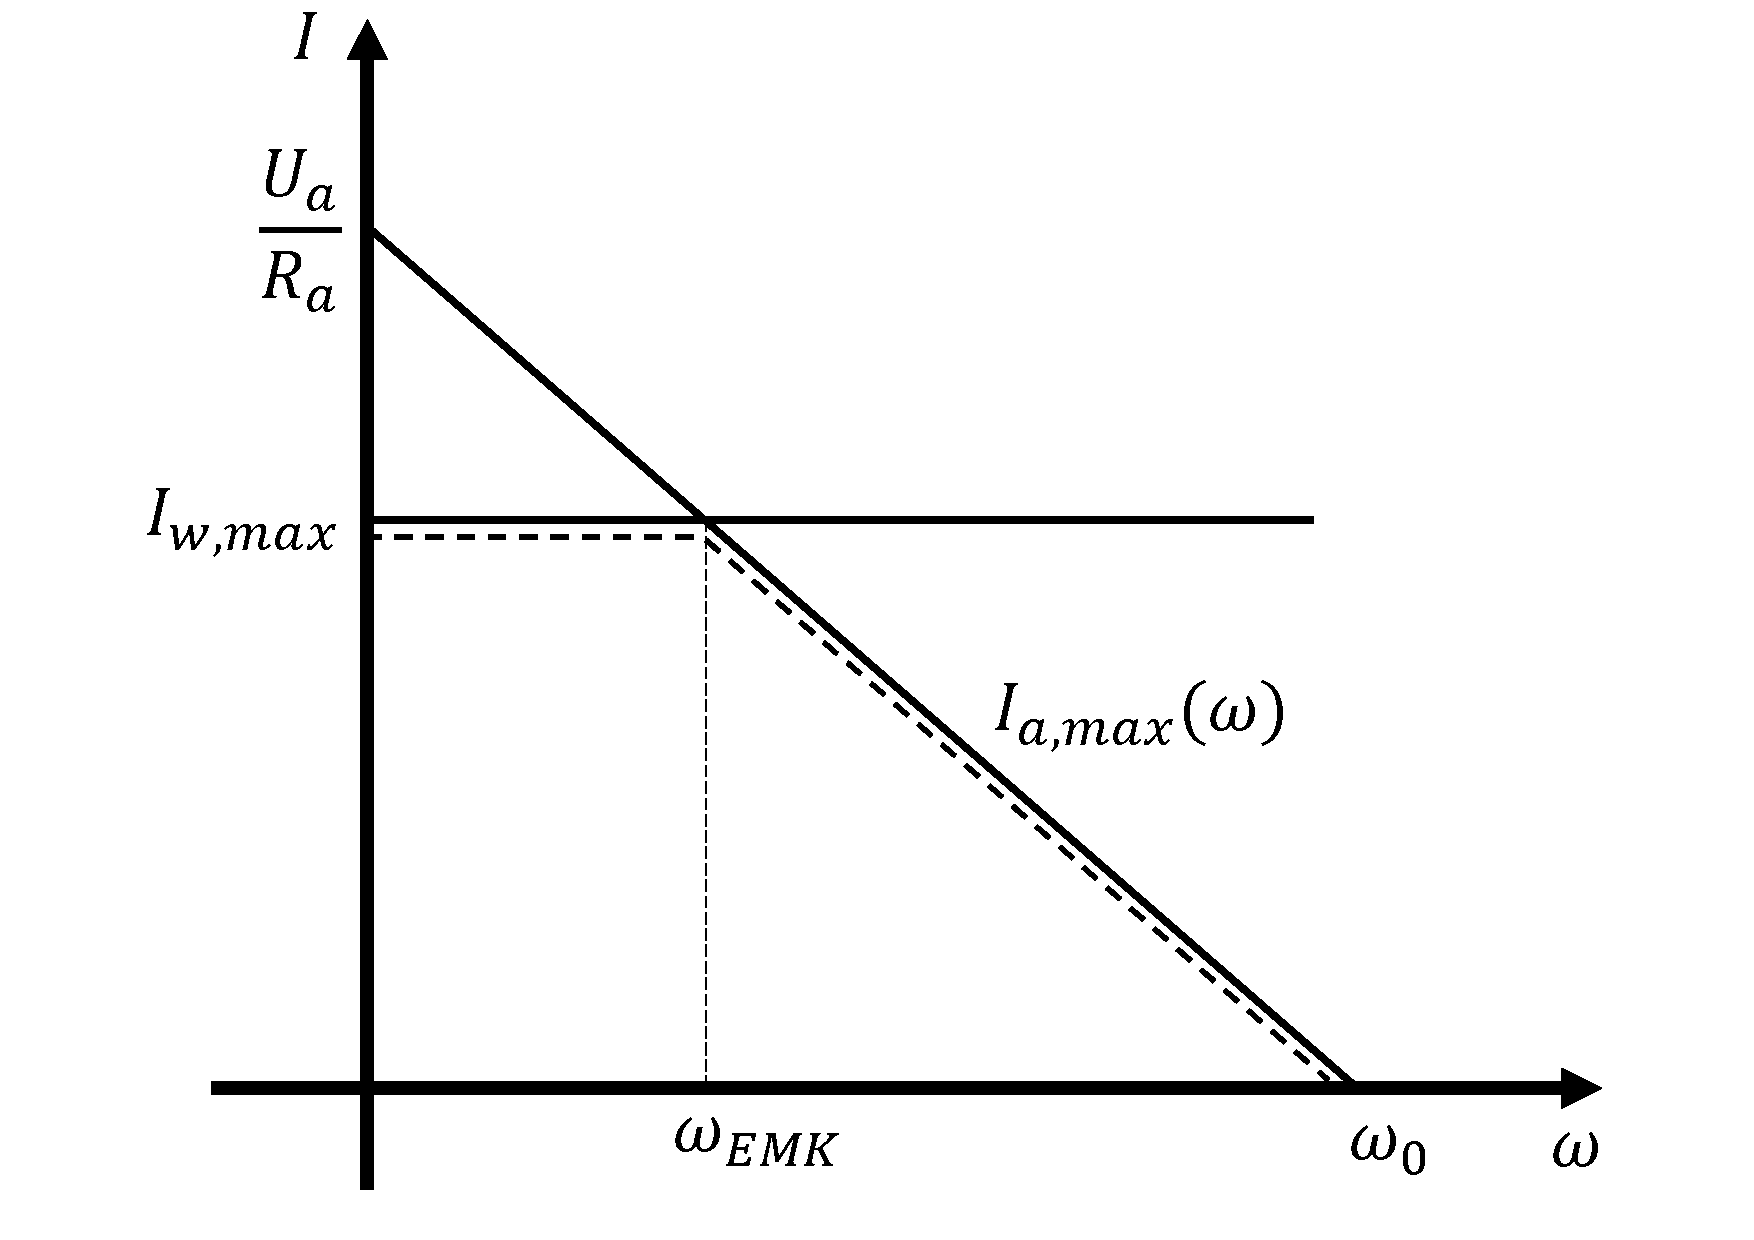
\includegraphics[width=0.50\textwidth]{Bilder/Motor/Stromkennlinie.pdf}
	\caption{Stromkennlinie}
	\label{fig:Stromkennlinie}
\end{figure}

Auf Grund der integrierten Strombegrenzung zum Schutz von Motor und Verstärker wird der vom Wandler bereitstellbare Strom zusätzlich begrenzt. Der dadurch parametrierte Maximalstrom des Wandlers wird durch den Stromregler zunächst konstant gehalten bis die Strombegrenzung der Gegen-EMK ab einer bestimmten Winkelgeschwindigkeit $\omega_{EMK}$ die des Wandler unterschreitet (siehe Abbildung /ref{fig:Stromkennlinie}). An dieser Stelle tritt ein "`Knick"' im Stromverlauf auf. Für den Stromregler wird dabei vereinfachend angenommen, über ausreichend hohe Dynamik und Stellenergie zu verfügen, um den Strom bis zur EMK-Grenze zu jedem Zeitpunkt konstant halten zu können.

Es werden zunächst nur positive Winkelgeschwindigkeiten betrachtet. 
Der Abschnitt des Verlaufs in Abbildung /ref{fig:Stromkennlinie} mit konstantem maximalen Strom wird durch

\begin{equation}
	I_a  = I_{w\mrm{, max}} = \mrm{const.} \ , \qquad 0 \leq \omega \leq \omega_{\mrm{EMK}}
	\label{eq:Iconst}
\end{equation}

beschrieben, wobei $I_{w\mrm{, max}}$ der Begrenzungsstrom des Wandlers ist.

\begin{figure}[h]
	\centering
		\begin{circuitikz}[european]
	\draw (0,0) 
		to[short, -, i=$I_a$] (1,0)
		to[R=$R$] (3.5,0)
		to[L=$L$] (6,0)
		to[V=$U_i$] (6,-2)
		-- (0,-2);
	\draw
		node[ocirc] (A) at (0,0) {}
		node[ocirc] (B) at (0,-2) {};
		%(A) to[open, v=$U_a$] (B);	
		\begin{scope}[shorten >= 10pt,shorten <= 10pt]
			\draw[->] (A) -- node[left] {$U_a$} (B);
		\end{scope}  
\end{circuitikz}
	\caption{Ersatzschaltbild eines Gleichstrommotors}
	\label{fig:dcESB}
\end{figure}

Der Verlauf des Bereichs mit zeitlich abnehmender maximaler Stromstärke wird aus dem Ersatzschaltbild des Gleichstrommotors in Abbildung \ref{fig:dcESB} hergeleitet. Aus dem zweiten Kirchhoffschen Gesetz (Maschenregel) ergibt sich

\begin{equation}
	U_a =  RI_a + L \frac{dI_a(t)}{dt} + U_i \ . 
	\label{eq:dcMasche}
\end{equation}

Für die Kennlinie des maximalen Stroms liegt der Tastgrad (engl.: \textit{duty cylcle}) der pulsweitenmodulierten Ankerspannung bei $100\%$, sodass 
\[
	U_{a \mrm{, max}},  = const.
\]
gilt. Die elektrische Zeitkonstante des Motors, die mit den Angaben des Datenblatts [???] zu 
\[
	\tau_{\mrm{el}} = \frac{L}{R} \approx 0,0023 << 1 \ ,
\]
berechnet werden kann, ist ausreichend klein, dass näherungsweise von stationärem Betrieb ausgegangen werden kann und für die selbstinduzierte Spannung 
\[
	L \frac{dI_a(t)}{dt} \approx 0
\]
gilt. Die induzierte Gegenspannung wird gemäß \cite{binder} durch Proportionalität zur Winkelgeschwindigkeit
\[
	U_i  = K_I \cdot \omega \ 
\]
modelliert.
Damit kann Gleichung \eqref{eq:dcMasche} zur Geraden

\begin{equation}
	I_{a \mrm{, max}}(\omega) = \frac{U_a}{R} - \frac{K_I}{R} \omega \ , \qquad \omega > \omega_{\mrm{EMK}} \ .
	\label{eq:Ivar}
\end{equation}

umgeformt werden.
Die Beschreibung des Bereichs negativer Winkelgeschwindigkeiten kann aus den Gleichungen \eqref{eq:Iconst} und \eqref{eq:Ivar} durch eine Punktspiegelung des in Abbildung \ref{fig:Stromkennlinie} dargestellten Verlaufs in den dritten Quadranten gewonnen werden.

Zusammenfassend ergibt sich aus \eqref{eq:Iconst} und \eqref{eq:Ivar} für den Verlauf des maximal verfügbaren Stroms  
\[
I_{a \mrm{, max}}(\omega) = \left\{\begin{array}{lll}
														-\frac{U_a}{R} - \frac{K_I}{R} \omega, & \omega < -\omega_{\mrm{EMK}}   \\ \\
														I_{w\mrm{, max}} \cdot \sign{\omega} 	& -\omega_{\mrm{EMK}} \leq \omega \leq \omega_{\mrm{EMK}} \\ \\				
														\frac{U_a}{R} - \frac{K_I}{R} \omega, & \omega > \omega_{\mrm{EMK}} \end{array}\right. . \
\] 

\subsection{Getriebe}

\begin{figure}[htbp]
	\centering
		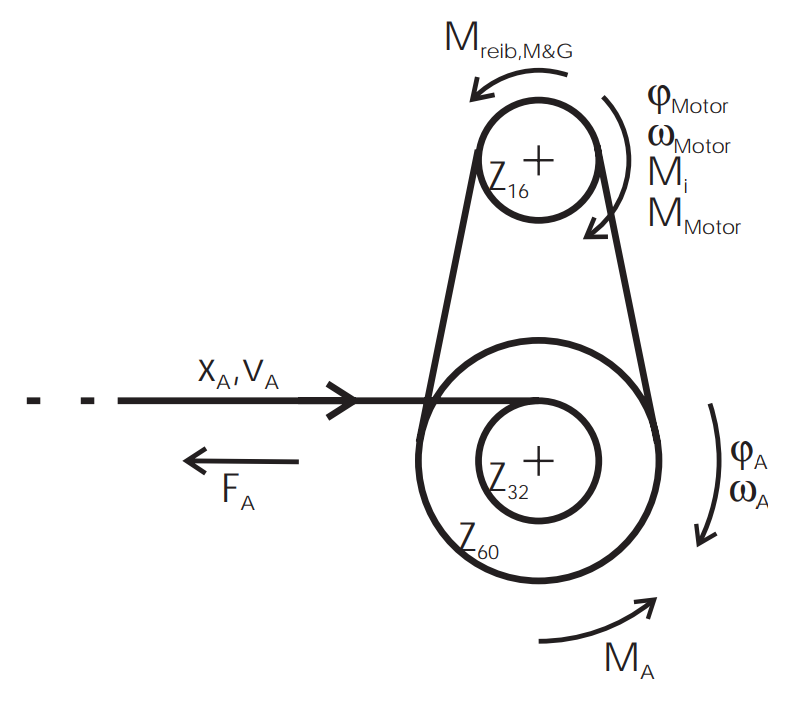
\includegraphics[width=0.5\textwidth]{Bilder/Motor/Getriebe.PNG}
	\caption{Getriebe \cite{franke}}
	\label{fig:Getriebe}
\end{figure}

Die Rotorbewegung des Motors wird über das in Abbildung \ref{fig:Getriebe} dargestellte Getriebe und das Antriebszahnrad auf den Zahnriemen weitergegeben. Auf Grund der hohen Steifigkeit des mit eingebetteten Stahlseilen unterstützten Riemens wird dieser wie in Apprich \cite{apprich} als unendlich starr angenommen, sodass die Verbindung von Motor und Schlitten ohne Federkopplung durch eine Übersetzungskonstante modelliert werden kann.
\[
	\dot{x} = K_G \cdot \omega
\]
 Die Übersetzungskonstante $K_G$ zwischen der Winkelgeschwindigkeit des Motors und der Schlittengeschwindigkeit wird über das Zahnverhältnis und den Antriebsradius berechnet.
\[
	K_G =  \frac{Z_{16}}{Z_{60}} \cdot r_{32} \ .
\]
Der Antriebsradius $r_{32}$ ist dabei der Abstand zwischen der neutralen Phase des Riemens und der Drehachse.